\paragraph{QuizziPedia::Front-End::Controllers::QuestionnaireManagementController}
\begin{figure} [ht]
	\centering
	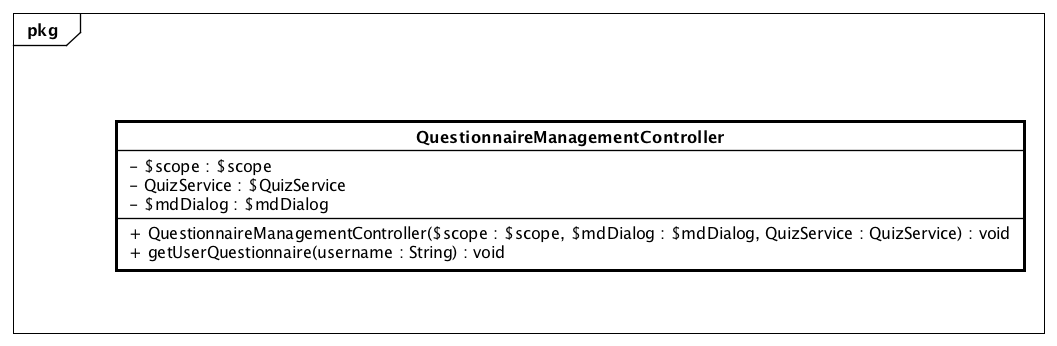
\includegraphics[scale=0.45]{UML/Classi/Front-End/QuizziPedia_Front-end_Controller_QuestionnaireManagementController.png}
	\caption{QuizziPedia::Front-End::Controllers::QuestionnaireManagementController}
\end{figure} \FloatBarrier
\begin{itemize}
	\item \textbf{Descrizione}: questa classe permette di gestire tutti i questionari creati da un utente; 
	\item \textbf{Utilizzo}: fornisce le funzionalità per recuperare dal back-end tutti i questionari creati da un utente;
	\item \textbf{Relazione con altre classi}:
	\begin{itemize}
		\item \textit{IN} \texttt{QuestionnaireManagementModelView}: ;
		\item \textit{IN} \texttt{QuizService}: questa classe permette di ottenere i dati di un quiz tramite delle parole chiave inserite dall'utente nella barra di ricerca;
		\item \texttt{-} \texttt{\$mdDialog: \$mdDialog} \\
		Campo dati contenente un riferimento al servizio della libreria \textit{Material for Angular\ped{G}} che permette di creare delle componenti a popup;
		\item \textit{IN} \texttt{QuestionnaireModel}: ;
	\end{itemize}
	\item \textbf{Attributi}:
	\begin{itemize}
		\item \texttt{-} \texttt{\$scope: \$scope} \\
		Campo dati contenente un riferimento all’oggetto \$scope creato da \textit{Angular\ped{G}}, viene utilizzato come mezzo di comunicazione tra il controller e la view. Contiene gli oggetti che definiscono il model dell’applicazione;
		\item \textit{IN} \texttt{QuizService}: permette di ottenere i dati di un quiz tramite delle parole chiave inserite dall'utente nella barra di ricerca;
		\item \texttt{+} \texttt{quizManagement: QuestionnaireManagementModelView} \\
		Oggetto di tipo \texttt{QuestionnaireManagementModelView}. All'interno di esso sono presenti le variabili e i metodi necessari per il \textit{Two-Way Data-Binding\ped{G}} tra la view \texttt{QuestionnaireManagementView} e il controller \texttt{QuestionnaireManagementController};
	\end{itemize}
	\item \textbf{Metodi}:
	\begin{itemize}
		\item \texttt{+} \texttt{QuestionnaireManagementController(\$scope: \$scope, \$mdDialog: \$mdDialog, QuizService: QuizService)}: \\Metodo costruttore della classe;\\
		\textbf{Parametri}: 
		\begin{itemize}
			\item \texttt{-} \texttt{\$scope: \$scope} \\
			Campo dati contenente un riferimento all’oggetto \$scope creato da \textit{Angular\ped{G}}. Viene utilizzato come mezzo di comunicazione tra il controller e la view. Contiene gli oggetti che definiscono il viewmodel e il model dell’applicazione;
			\item \texttt{-} \texttt{\$mdDialog: \$mdDialog} \\
			Campo dati contenente un riferimento al servizio della libreria \textit{Material for Angular\ped{G}} che permette di creare delle componenti a popup;
			\item \texttt{-} \texttt{QuizService: QuizService}: parametro che permette di ottenere, tramite il service, la lista di tutte le domande presenti nel quiz;
		\end{itemize}
		\item \texttt{-} \texttt{getUserQuestionnaire(username: String) QuestionnaireModel[]}: \\Metodo che ritorna tutti i questionari creati da un utente in un array di QuestionnaireModel.
		\textbf{Parametri}:
		\begin{itemize}
			\item \texttt{username: String}: parametro che indica l'identificativo dell'utente del quale vogliamo scaricare tutti i questionari.
		\end{itemize}
	\end{itemize}
\end{itemize}

